\chapter{Le framework Mechanics, Dynamics, Aesthetics}

La conception de jeu est le processus de réflexion nécessaire à la création d'un jeu vidéo ou de n'importe quelle sorte de jeu. C'est le chemin que suit le jeu depuis une idée jusqu'à sa réalisation. De nombreuses étapes permettent de mettre en place tous les aspects du jeu pour le mener à sa version jouable. La mise en place du monde dans lequel le joueur évoluera, les règles qu'il devra suivre pour avancer, les éléments graphiques qu'il rencontrera tout cela est définit lors de la conception. Le jeu vidéo est cependant difficile à concevoir et surtout à documenter. Un logiciel classique répond au besoin d'un utilisateur qui s'en sert pour résoudre une problématique. Un jeu quant à lui doit apporter un but au le joueur, l'envie de continuer à l'utiliser et générer donc des émotions pour être apprécié. Il est très compliqué de définir une méthodologie précise pour décrire une émotion générée ainsi que tous les éléments techniques autour d'un jeu vidéo. C'est ce que le Framework \gls{mda} propose.


\section{Le jeu comme un échange entre Game Designer et Joueur}
Un Game Designer créé un jeu dans le but de générer une expérience de jeu.
\begin{figure}[H]
    \centering
    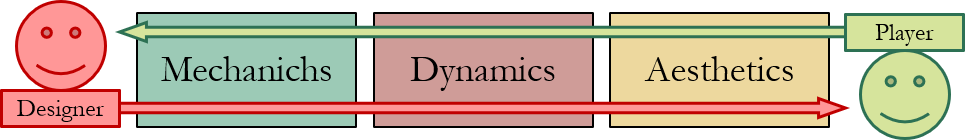
\includegraphics[width=14cm]{10_img/chap3/mda.png} 
    \caption{Contenu des parties du Framework MDA \cite{MDA_formal}}
\end{figure}


%MDA: A Formal Approach to Game Design and Game Research Robin Hunicke, Marc LeBlanc, Robert Zubek
%A better recipe for game jams: using the Mechanics Dynamics Aesthetics framework for planning Paris Buttfield-Addison,Jon Manning,Tim Nugent
%\Design, Dynamics, Experience (DDE): An Advancement of the MDA Framework for Game Design
\section{Mechanics}
[Leblanc ppt] Mechanics = code + rules / Game as system
Représentation des datas et algorithmes
Tous les objets et les mécaniques de jeux (level design, gameplay...).
Toutes les actions, comportements et controles attribués au joueur.
Il existe beaucoup de méchanics de jeu (cards, shooter, golf...)
Certains comportement sont des conséquences directes des règles = mechanics



\section{Dynamics}
[Leblanc ppt] Dynamics Process + Game "session"
Mechanics et Dynamics sont différentes view du jeu
Les Dynamics découlent des Mechanics
Certains comportement sont des conséquences indirectes des règles = Dynamics
Comportement au runtime
Partie des mechanics que le joueur peut voir: qu'est ce qu'il se passe quand le joueur appuie sur un bouton, qu'est ce qu'il se passe quand il effectue une action 
Qu'est ce qui est prédictible et explicable concernant le comportement du jeu ?
Il est possible d'analyser les autres jeux mais également : utiliser les calculs des autres jeux (maths), étudier la psychologie du joueur...



\section{Aesthetics}
[Leblanc ppt] Aesthetics Requirements + fun
représente les émotions générées pour le joueur quand il intéragit avec le systeme
Passe par tous les sens atteignables et les émotions
8 sortes de "fun"(Jeu pour le) : sensation (plaisir des sens), fantasy (make-believe), narrative(drama), challenge(suite d'obstacles), fellowship(réseau social), discovery(territoires inconnus), expression(découverte de soi meme), submission(passe temps).
Chaque jeu peut contenir un ou plusieurs types de fun
L'aesthetics peut etre un objectif dans le développement d'un jeu




\section{Les limitations et évolutions possibles}
\subsection{DPE : Le Framework Design, Play, Experience}
%ARTCILE The Design, Play, and Experience Framework, Brian M. Winn
DPE (Design Play Experience framework pour designer les serious games
Approche formelle pour diesigner l'apprentissage, le story telling, le gameplay, l'experience utilisateur et les composants techno d'un jeu sérieux
DPE est une extension du MDA

\begin{figure}[H]
    \centering
    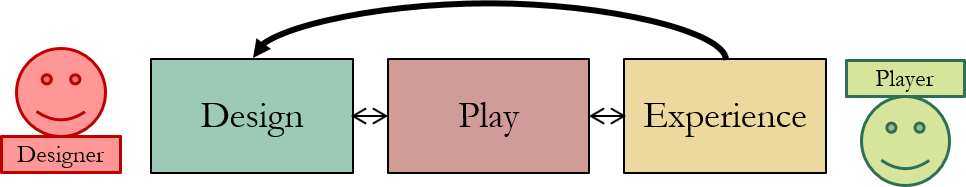
\includegraphics[width=10cm]{10_img/chap3/dpe.png} 
    \caption{Contenu des parties du Framework DPE \cite{Winn2011}}
\end{figure}

Le designer design le jeu, le joueur y joue, ce qui créé l'expérience.
Le designer a le contrôle direct sur tout le design. Pour cela il doit définir des objectifs d'expérience (c'est ce que représente la flèche depuis Experience vers Design). Cette flèche représente aussi le processus itératif du design (Salen et Zimmermann 2004) Le design entraîne un prototype, l'expérience sur ce prototype permet de revoir le design.

\begin{figure}[H]
    \centering
    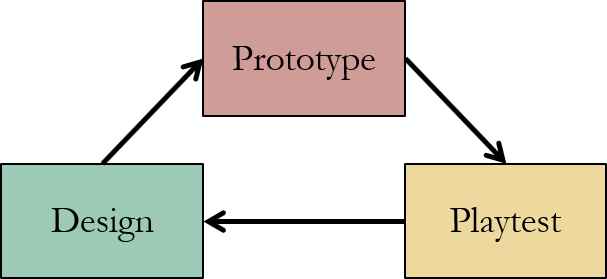
\includegraphics[width=8cm]{10_img/chap3/iteration_prototype.png} 
    \caption{Processus de design itératif \cite{Winn2011}}
\end{figure}

\begin{figure}[H]
    \centering
    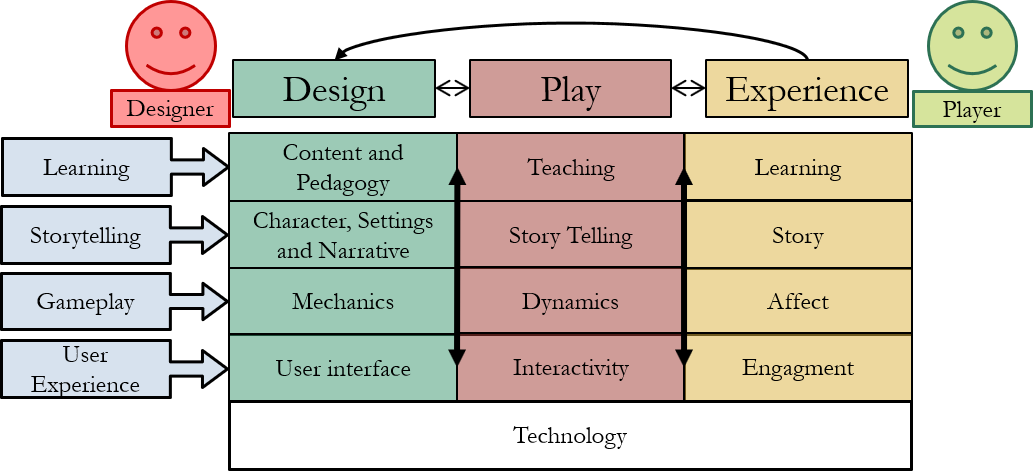
\includegraphics[width=14cm]{10_img/chap3/dpe_extended.png} 
    \caption{Framework DPE étendu \cite{Winn2011}}
\end{figure}



\subsection{DDE : Le framework Design, Dynamics, Experience \cite{DDE}}
%ARTICLE DDE Design, Dynamics, Experience (DDE): An Advancement of the MDA framework for Game Design Wolfgang

%GAMASUTRA From MDA to DDE, Wolfgang Walk
Néglige beaucoup d'aspects de design des jeux vidéos
Se concentre trop sur les méacaniques
Ne convient pas à tous les types de gameplay (jeux sérieux, gamification, narrative
Schell introduit des notions de Story et Technologies, alliées à la méecanique et aesthetics du MDA. 
Dans le MDA le designer n'a que peu de controle sur les dynamics et aesthetics car ceux ci decoulent que des mecaniques décrites avant.

\begin{figure}[H]
    \centering
    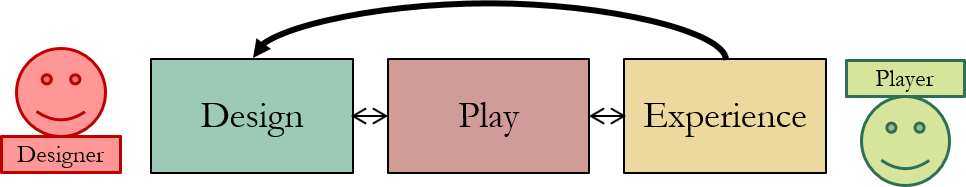
\includegraphics[width=10cm]{10_img/chap3/dpe.png} 
    \caption{Contenu du Framework DDE \cite{DDE}}
\end{figure}

%MODIFIER LE GRAPHIQUE POUR LES BONS TITRES !!!!!!!!!!!!!!!!!!!!!!!!!!!!
\begin{figure}[H]
    \centering
    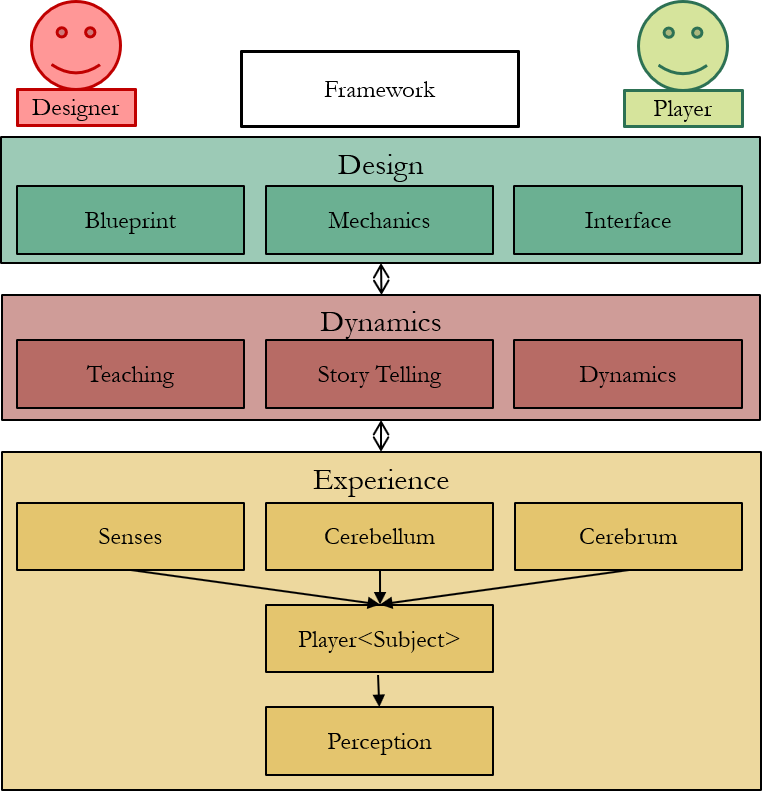
\includegraphics[width=14cm]{10_img/chap3/dde_extended_modif.png} 
    \caption{Framework DDE étendu \cite{DDE}}
\end{figure}

\subsubsection{Design}
    \begin{itemize}
        \item Blueprint : Partie du design qui concerne les concepts du monde du jeu : culture, religionm physique, les différents sets de règles, les styles artistiques, le design narratif, le design de personnages et le design sonore qui ensemble créés l'expérience esthétique.
        \item Mechanics : Toute chose créant le jeu, plus précisément le code. L'architecture du code, la prise en charge des entrées/sorties, la prise en charge des objets, l'implémentation des règles de jeu et l'interaction entre les objets, et tous les éléments reliés au code. Cela comprend tous les éléments que le joueur ne perçoit pas dans son utilisation du jeu.
        \item Interface : Toutes les mécaniques qui ont pour but de communiquer le jeu au joueur. Les graphismes, le son, les reéactions et interactions entre le joueur et le jeu, ainsi que celles bouclant sur le jeu lui-même. Cette partie comprend également les cinématiques les textes affichés et tout ce qu'il est possible de voir ou d'entendre dans le jeu.
    \end{itemize}

\subsubsection{Dynamics}
    La catégorie Dynamics du DDE correspond à celle présente dans le MDA, mais elle classifie les interactions de manière à les rendre plus précises. Cest ainsi que ces Dynamics se retrouvent en trois grande catégories: Player <-> Game, Player <-> Player et Game <-> Game.

\subsubsection{Experience}
    Dans le MDA la troisième partie du framework est l'Aesthetics : tout ce que le joueur sent et ressent lors de son activité sur le jeu. La partie Experience du jeu étend l'Aesthetics afin de prendre en considération que le joueur n'est pas une somme des émotions générées par le jeu, mais également un élément avec une expérience déjà présente avant l'utilisation du jeu qui peut modifier les émotions générées d'un joueur à l'autre. Une même couleur, un même son ou une même image peuvent générer différentes réactions de la part du joueur et la partie Experience du DDE essaie de prendre en compte cela.
    \begin{itemize}
        \item Senses: expérience sensorielle du joueur du début à la fin du jeu.
        \item Cerebellum : Les émotions ressenties par le joueur.
        \item Cerebrum : Les challenges intellectuels et les décisions prises par le joueur.
        \item Player<Subject> : Partie que le designer ne peut pas controller. Il peut se base sur les trois premières catégories afin de prévoir une réponse spécifique du joueur, mais n'ayant aucun contrôle sur celle-ci il ne peut que estimer la réaction du joueur en fonction d'objectifs et de logiques psychologiques pour l'amener à la réaction souhaitée.
        \item Perception : Ce que ressent réellement le joueur en focntion des 3 première catégories et de sa propre expérience et personnalité en tant que joueur. Cela comprendra son gameplay, le type de challenge qu'il perçoit, l'amusement qu'il ressent, la beauté qu'il perçoit, l'échos que génère l'histoire en lui, etc.
    \end{itemize}


%GAMASUTRA Revisiting the MDA framework, Luiz Claudio Silveira Duarte
\subsection{Le MDA est limités à la représentation des jeux vidéos}
Dans son article Duarte \cite{GAMA_MDA} met en avant des limitations que le MDA a à représenter des jeux qui ne soient pas des Jeux vidéos. Il explique que les règles d'un jeu vidéo sont souvent implicites au type de gameplay ou de genre de classification de jeu vidéos. Cependant dans le cadre des jeux de plateau les règles ne peuvent pas être implicites et acquises par l'expérience, elles doivent être explicites et explicables dans un manuel d'utilisation. Il fait l'analogie entre un FPS (First Personnal Shooter) et un jeu d'échecs. Dans un FPS un joueur sait à quoi s'attendre dans le genre de jeux selon son expérience du genre, il saura ou trouver les éléments et saura comment faire usage de l'interface graphique qui lui est présentée. Cependant un joueur se retrouvant devant un jeu d'échec pour la première fois ne pourra pas acquérir les connaissances requises pour jouer par l'expérience, les règles devront lui être expliquées à la base et l'expérience ne pourra lui apporter que des aspects tactiques du jeu.